\section{Auswertung}

Ausgleichsrechnungen mit Fehlerfortpflanzung werden mit scipy.optimize.curve\_fit aus dem Programm
Python durchgeführt.

\subsection{Kontrast}

Fit nach der Funktion
\[
K = a \cdot | \sin (2 \cdot \phi + b) |
\]
liefert die Fitparameter $a = 1.06 \pm 0.05$ und $b = 1 \pm 2$

\begin{figure}[h]
\centering
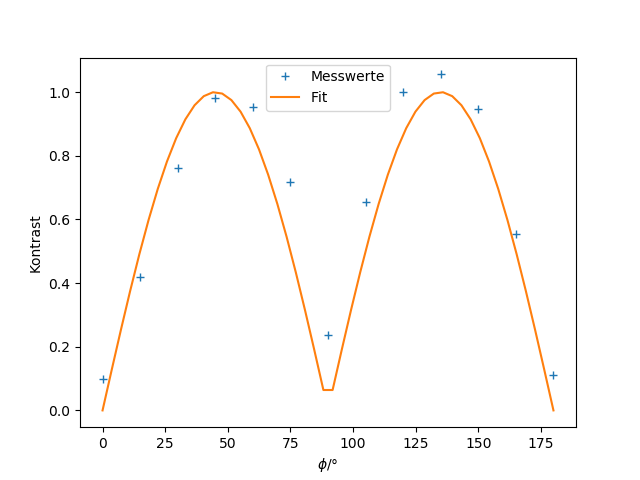
\includegraphics[width=\linewidth]{img/kontrast.png}
\caption{Ausgleichsrechnung für den Zusammenhang zwischen dem Winkel $\phi$ und dem Kontrast $K$.}
\label{kontrast}
\end{figure}

\subsection{Brechungsindex von Glas}

Fit nach der Funktion in Gleichung (\ref{glas})
liefert den Fitparameter $a = 1.553 \pm 0.009$, was auch bereits der Brechungsindex von Glas ist.

\begin{figure}[h]
\centering
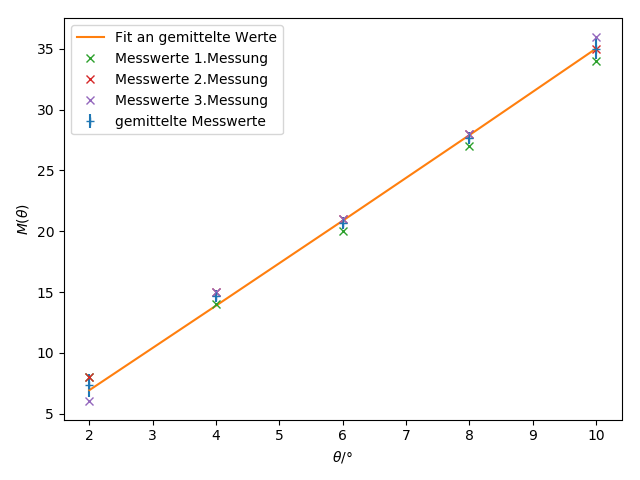
\includegraphics[width=\linewidth]{img/n_glas.png}
\caption{Lineare Ausgleichsrechnung für den Zusammenhang zwischen dem Winkel $\theta$ und der Anzahl
der Intensitätsmaxima.}
\label{n_glas}
\end{figure}

\subsection{Brechungsindex von Luft}

Fit nach der Funktion
\[
n = \sqrt{a \cdot p + 1}
\]
liefert den Fitparameter $a = 6.05 \cdot 10^{-7} \pm 4 \cdot 10^{-9}$

Daraus ergibt sich für den Brechungsindex bei Normalbedingungen: $0.999547 \pm 0.000003$.

\begin{figure}[h]
\centering
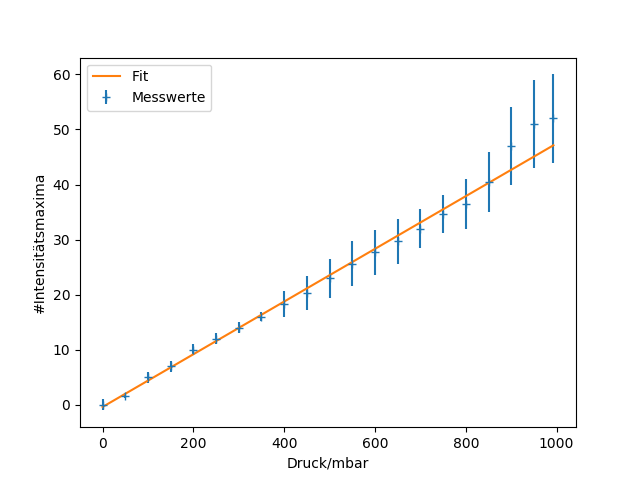
\includegraphics[width=\linewidth]{img/n_luft.png}
\caption{Lineare Ausgleichsrechnung für den Zusammenhang zwischen dem Druck $p$ und dem Brechungsindex.}
\label{n_luft}
\end{figure}
